\chapter{Аналитический раздел}
В данном разделе будут рассмотрены теоретически основы работы данных выше алгоритмов сортировки ''пузырьком'', алгоритмов сортировки ''расчёской'', алгоритм сортировки вставками.

\section{Основные сведения об алгоримтах}
Сортировка является одной из операций, которые необходимы при работе над данным. В частности эта необходимость возникает из-за потребности какой-либо обработки данных в процессе выполнения программы. Входные параметры варьируются от сортировке к сортировке, однако в общем случае на вход подаётся массив данных, а на выходе алгоритм возвращает отсортированный определённым образом массив.

\section{Алгоритм сортировки ''пузырьком''}
Данный алгоритм работает за счёт повторяющихся проходов по массиву, который был подан на вход. При каждом проходе последовательно сравниваются два соседних элемента. Если порядок в паре не соответствует условию сортировки, то элементы являются местами. Всего проходов по массиву выполняется N - 1 раз, где N - длина массива. При каждом проходе по внутреннему циклу алгоритм находит наибольший элемент и помещает его рядом с предыдущим наибольшим элементом, который был найден во время предыдущего прохода, а наименьший элемент, перемещается на одну позицию в сторону начала массива, если сортировка идёт по возврастанию. 

\section{Алгоритм сортировки ''расчёской''}
Основная идея данного алгоритма залючается в том, что при каждом проходе сравниваются элементы, находящиеся на неком расстоянии. Использование данного приёма позволяет быстро перемещать элементы из разных концов массива, избегая появления ''черепах'' - элементов, которые долго переходят из одного конца массива в другой. В остальных отношениях данный алгоритм работает аналогично сортировке ''пузырьком''. Расстояние между сравниваемыми величинами изменяется от N - 1, до 0.

\section{Алгоритм сортировки вставками}
Основная идея сортировки вставками состоит в том, что при сортировке элементы сгоняются в один из концов массива, являющийся отсортированным подмассивом. Это позволяет при каждом проходе сразу вставлять элемент в нужное место в уже отсортированную часть массива. Массив считается отсортированным, когда отсортированная часть поглощает весь массив.

\section{Модель вычислений}
Для того, чтобы вычислить трудоёмкость алгоритма, введём следующую модель вычислений:

\begin{enumerate}
	\item операторы, трудоёмкость которых равна 1: +, -, /, \%, ==, !=, <, >, >=, <=, [], ++;
	\item трудоёмкость оператора выбора if (условие) then A else B рассчитывается как $f_{\text{условия}} + f_{A}$ или $f_{B}$ в зависимости то того, какое условие выполняется;
	\item трудоёмкость цикла рассчитывается как $f_{for} = f_{\text{инициализации}} + f_{\text{сравнения}} + N(f_{\text{тела}} + f_{\text{инициализации}} + f_{\text{сравнения}})$;
	\item трудоёмкость вызова функции равна 0.
\end{enumerate}

\section{Вывод}
В данном разделе были рассмотрены основные теоретические сведения об алгоритме сортировки ''пузырьком'', алгоритме сортировки ''расчёской'', алгоритме сортировки вставками. В результате были сделаны выводы о том, что на вход алгоритму подаётся несортированный массив, на выходе программа возвращает отсортированный массив. Алгоритмы работают на массивах с размерностями от 0 до физически возможного предела для изпользуемой машины. В качестве критерия для сравнения эффективности алгоритмов будет использоваться время работы на массивах различного размера. Помимо этого был проведён анализ модели вычислений, которая будет использоваться трудоёмкости алгоритмов.

\chapter{Конструкторский раздел}

В данном разделе будут рассмотрены схемы, структуры данных, способы тестирования, описания памяти для следующих алгоритмов:
\begin{enumerate}
	\item алгоритм сортировки ''пузырьком'';
	\item алгоритм сортировки ''расчёской'';
	\item алгоритм сортировки вставками.
\end{enumerate}

\section{Тестирование алгоритмов}

Описание классов эквивалентности:
\begin{enumerate}
	\item проверка работы на пустом массиве;
	\item проверка работы на общем случае.
\end{enumerate}

Описание тестов:
\begin{enumerate}
	\item тест на пустом массиве - на вход подаётся пустой, выход сравнивается с пустым массивом;
	\item тест на общем случае - на вход подаётся массив длиной n, выход сравнивается с отсортированной версией массива, поданного на вход.
\end{enumerate}

\section{Алгоритм сортировки ''пузырьком''}

Алгоритм сортировки "пузырьком" реализуется по описанным выше принципам. На вход подаётся сортируемый массив, на выходе получается отсортированный массиы.

Используемые типы и структуры данных включают в себя:
\begin{enumerate}
	\item integer, целое число - используется для хранения индексов массива, размера массива;
	\item bool, логическая переменная - используется для хранения флага;
	\item array, массив целых чисел - используется для хранения серии целых чисел.
\end{enumerate}

\newpage

\begin{figure}[ph!]
	\center{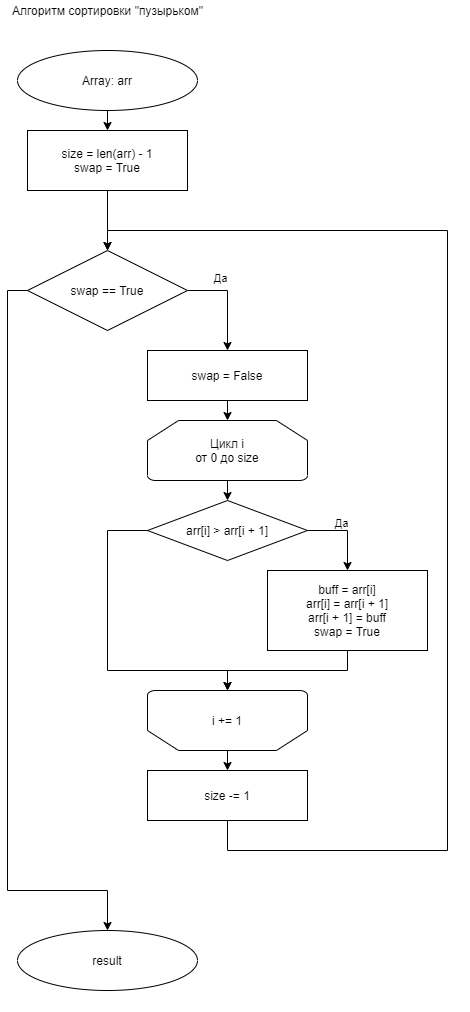
\includegraphics[scale=0.6]{bubble_scheme}}
	\caption{Схема алгоритма сортровки ''пузырьком''}
\end{figure}

\section{Алгоритм сортировки ''расчёской''}

Используемые типы и структуры данных включают в себя:
\begin{enumerate}
	\item integer, целое число - используется для хранения индексов массива, размера массива;
	\item float, вещественное число - используется для хранения коэффициента;
	\item bool, логическая переменная - используется для хранения флага;
	\item array, массив целых чисел - используется для хранения серии целых чисел.
\end{enumerate}

\newpage
\begin{figure}[ph!]
	\center{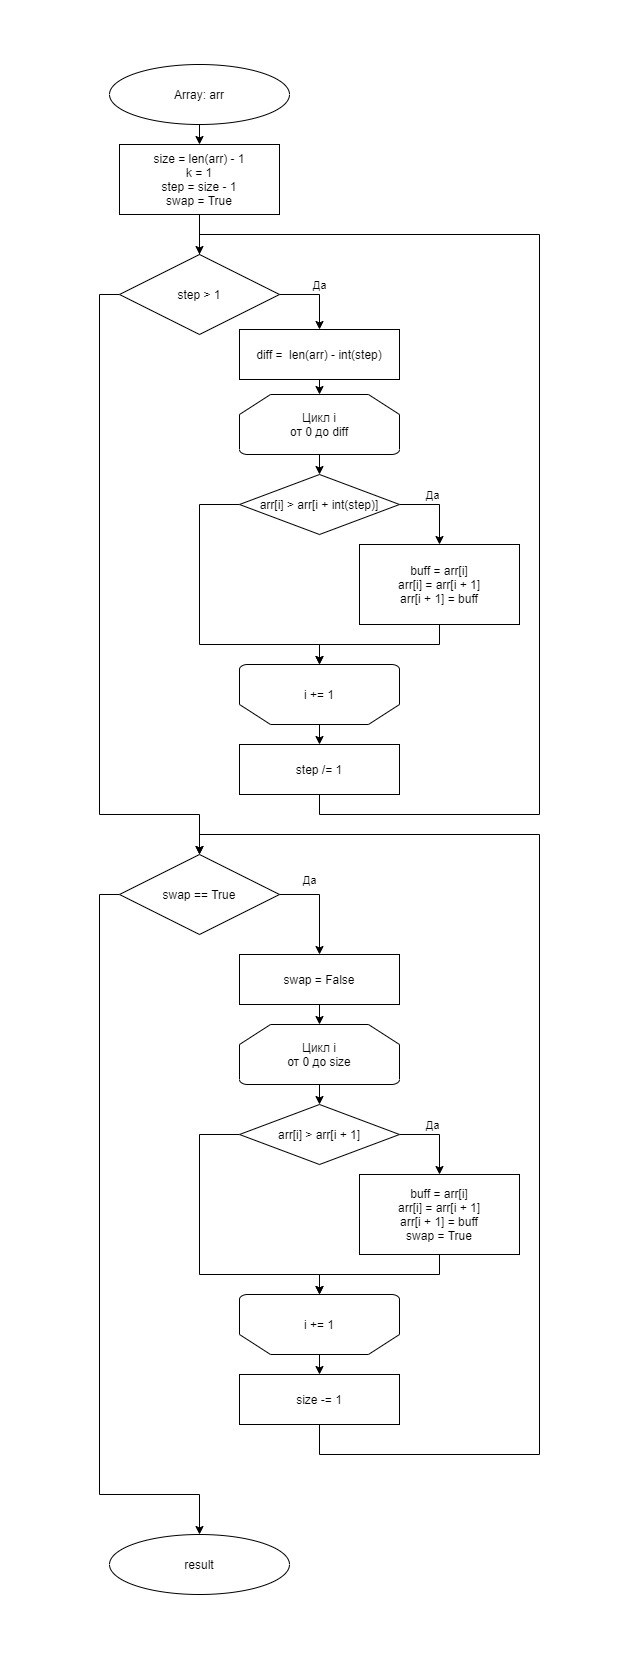
\includegraphics[scale=0.5]{comb_scheme}}
	\caption{Схема алгоритма сортировки ''расчёской''}
\end{figure}

\section{Алгоритм сортировки вставками}

Используемые типы и структуры данных включают в себя:
\begin{enumerate}
	\item integer, целое число - используется для хранения индексов и размерностей матрицы
	\item matrix, массив массивов вещественного типа - используется для хранения двух входных матриц и матрицы, хранящей результат умножения
\end{enumerate}

\newpage
\begin{figure}[ph!]
	\center{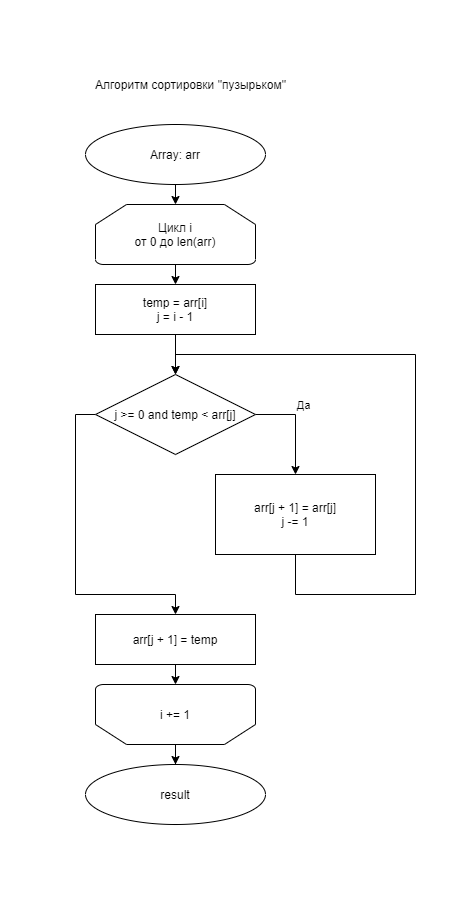
\includegraphics[scale=0.6]{insert_scheme}}
	\caption{Схема алгоритма сортировки вставками}
\end{figure}

\section{Трудоёмкость алгоритмов}
Проведём оценку трудоёмкости алгоритмов на основе описанных выше схем. N - размер подаваемого на вход массива.

\begin{itemize}
	\item Трудоёмпость алгоритма сортировки ''пузырьком'':
	\begin{itemize}
		\item Лучший случай:
		\begin{itemize}
			\item Трудоёмкость - 2 + 1+ 1 + 1 + 3 + (N - 1)(3 + 4) + 1;
			\item Результирующая трудоёмкость - 7N + 2;
		\end{itemize}
		\item Худший случай:
		\begin{itemize}
			\item Трудоёмкость - 2 + 1 + 1 + (N - 1)(3 + 1 + (N/2)(4 + 2 + 4 + 3 + 1) + 1);
			\item Результирующая трудоёмкость - 7$N^2$ - 2N - 1;
		\end{itemize}
	\end{itemize}
	
	\item Трудоёмпость алгоритма сортировки ''расчёской'':
	\begin{itemize}
		\item Лучший случай:
		\begin{itemize}
			\item Трудоёмкость - 2 + 1 + 2 + (N/2)(1 + 2 + 3 + 4(N/2) + 1) + 1 + 1 + 1 + 1 + 3 + (N/2)(3 + 4) + 1;
			\item Результирующая трудоёмкость - $N^2$ + 7N + 21;
		\end{itemize}
		\item Худший случай:
		\begin{itemize}
			\item Трудоёмкость - 5 + (N/2)(1 + 2 + 3 + (N/2)(3 + 4 + 2 + 4 + 3) + 1) + 1) + 1 + 1 + 1 + 3 + (N/2)(3 + 4) + 1;
			\item Результирующая трудоёмкость - 4$N^2$ + 13N/2 + 12;
		\end{itemize}
	\end{itemize}

	\item Трудоёмпость алгоритма сортировки вставками:
	\begin{itemize}
		\item Лучший случай:
		\begin{itemize}
			\item Трудоёмкость - 3 + (N - 1)(2 + 2 + 4 + 4 + 4 + 1 + 1);
			\item Результирующая трудоёмкость - 18N - 5;
		\end{itemize}
		\item Худший случай:
		\begin{itemize}
			\item Трудоёмкость - 3 + (N - 1)(2 + 2 + 4 + (N/2)(4 + 4+ 1) + 1);
			\item Результирующая трудоёмкость - 9$N^2$/2 + N/2 -2;
		\end{itemize}
	\end{itemize}
\end{itemize}

\section{Функциональная схема ПО}
На изображении ниже представлена функиональная схема разрабатываемого ПО. На вход подаётся массив с числами и при помощи алгоритмов, реализованных на языке Python мы получаем в результате работы новый массив, содерждащий в себе результат сортировки.

\begin{figure}[ph!]
	\center{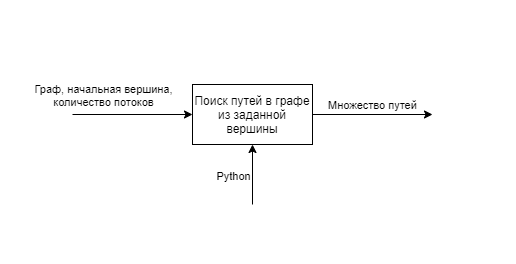
\includegraphics[scale=1.0]{func_scheme}}
	\caption{IDEF0 диаграмма разрабатываемой программы}
\end{figure}

\section{Вывод}
В данном разделе были рассмотрены схемы алгоритмов для каждого из алгоритмов сортировки, и были определены тесты для каждого алгоритма, были описаны типы и структуры данных, использующихся в алгоритмах. Также была произведена оценка трудоёмкости для изучаемых алгоритмов и приведена функциональная схема разрабатываемого ПО.

\chapter{Технологический раздел}

В данном разделе будут рассмотрены подробности реализации описаных выше алгоритмов. Также будут обоснованы выбор языка программирования для реализации, выбор библиотек для проведения экспериментов и представлены важные фрагменты кода написанной в рамках работы программы.

\section{Выбор языка программирования}

В качестве языка программирования для реализации данной лабораторной работы использовался язык программирования python (3.9.7) в целях упрощения работы со структурами данных и визцализацией данных сравнительных анализов и наличием опыта работы с данным языком программирования. В качестве среды разработки использовалась Visual Studio Code. 

\section{Сведения о модулях программы}

Реализованное ПО состоит из трёх модулей:
\begin{enumerate}
	\item algos.py - в данном модуле реализованы алгоритмы сортировки;
	\item time.py- в данном модуле реализованы замеры временных характеристик алгоритмов;
	\item tests.py - в данном модуле реализованы тесты алгоритмов.
\end{enumerate}

\section{Реализация алгоритмов сортировки массивов}

\begin{lstlisting}[label=some-code-1,caption=Реализация алгоритма сортировки ''пузырьком'']
def bubble_sort(arr):
  size = len(arr) - 1
  swap = True
  while swap:
    swap = False
    for i in range(0, size):
      if arr[i] > arr[i + 1]:
        buff = arr[i]
        arr[i] = arr[i + 1]
        arr[i + 1] = buff
        swap = True
    size -= 1
  return arr
\end{lstlisting}


\begin{lstlisting}[label=some-code-1,caption=Реализация алгоритма сортировки ''расчёской'']
def comb_sort(arr):
  size = len(arr) - 1
  k = 1
  step = size - 1
  while step > 1:
    diff = len(arr) - int(step)
    for i in range(0, diff):
      if arr[i] > arr[i + int(step)]:
        buff = arr[i]
        arr[i] = arr[i + 1]
        arr[i + 1] = buff
    step -= k
  swap = True
  while swap:
    swap = False
    for i in range(0, size):
      if arr[i] > arr[i + 1]:
        buff = arr[i]
        arr[i] = arr[i + 1]
        arr[i + 1] = buff
        swap = True
    size -= 1
  return arr 	
\end{lstlisting}

\begin{lstlisting}[label=some-code-1,caption=Реализация алгоритма сортировки вставками]
def insert_sort(arr):
  for i in range(1, len(arr)):
    temp = arr[i]
    j = i - 1
    while (j >= 0 and temp < arr[j]):
        arr[j + 1] = arr[j]
        j -= 1
    arr[j + 1] = temp
  return arr
\end{lstlisting}


\section{Реализация тестирования алгоритмов}

Для тестирования алгоритмов было реализованы следующие тесты:
\begin{enumerate}
	\item тест на нулевых масссивах;
	\item тест на массивов, заполненных рандомными величинами от -100 до 100 длиной n;
\end{enumerate}

\begin{lstlisting}[label=some-code-5,caption=Реализация функции рандомной генерации массивов]
def check_arr(arr_a, arr_b):
    res = True
    l = len(arr_a)
    for i in range(0, l):
        if arr_a[i] != arr_b[i]:
            res = False
    return res
\end{lstlisting}

\begin{lstlisting}[label=some-code-6,caption=Реализация общей функции тестирования]        
def test_case(arr_a, arr_true, case_name):
    print(case_name)
    print('Параметры массива: N = ', len(arr_a))

    res_bubble = bubble_sort(arr_a)
    res_comb = comb_sort(arr_a)
    res_insert = insert_sort(arr_a)

    print('Результат сортировки: ')
    print(arr_a)
    print(res_bubble)
    print(res_comb)
    print(res_insert)

    print("Проверка совпадения результатов: ")
    print(check_arr(arr_true, res_bubble))
    print(check_arr(arr_true, res_comb))
    print(check_arr(arr_true, res_insert))
    print('===\n')
\end{lstlisting}

\begin{lstlisting}[label=some-code-7,caption=Реализация тестов]      
arr_a = generate_random_test_array(5)
arr_true = arr_a.copy()
arr_true.sort()
test_case([], [], 'Нулевой массив')
test_case(arr_a, arr_true, 'Общий случай')
\end{lstlisting}

\section{Вывод}
В данном разделе была представлена реализация алгоритма сортировки ''пузырьком'', алгоритма сортировки ''расчёски'' и алгоритма сортировки вставками. Были разработаны алгоритмы тестирования разработанных методов по методу чёрного ящика.

\chapter{Экспериментальный раздел}

В данном разделе будут измерены временные характеристики алгоритмов умножения матриц и сделаны выводы об их временной эффективности.

\begin{table}[h!]
  \begin{center}
    \captionsetup{justification=raggedright}
    \caption{Время работы алгоритма сортировки ''пузырьком''}
    \label{tab:workcost_classic}
    \begin{tabular}{c|c}
      \textbf{Размерность массива} & \textbf{Время сортировки}\\
      \hline
	100 & 0.0\\
	250 & 0.0\\      
	500 & 0.015625\\ 
	750 & 0.03125\\  
	1000 & 0.03125\\ 
	1250 & 0.046875\\
	1500 & 0.078125\\
	1750 & 0.09375\\ 
	2000 & 0.140625\\
	2250 & 0.171875\\
	2500 & 0.234375\\
    \end{tabular}
  \end{center}
\end{table}

\begin{table}[h!]
  \begin{center}
    \captionsetup{justification=raggedright}
    \caption{Время работы алгоритма сортировки ''расчёской''}
    \label{tab:workcost_classic}
    \begin{tabular}{c|c}
      \textbf{Размерность массива} & \textbf{Время сортировки}\\
      \hline
	100 & 0.0\\      
	250 & 0.0\\      
	500 & 0.046875\\
	750 & 0.09375\\
	1000 & 0.15625\\
	1250 & 0.28125\\
	1500 & 0.390625\\
	1750 & 0.515625\\
	2000 & 0.703125\\
	2250 & 0.796875\\
	2500 & 1.03125\\
    \end{tabular}
  \end{center}
\end{table}

\begin{table}[h!]
  \begin{center}
    \captionsetup{justification=raggedright}
    \caption{Время работы алгоритма сортировки ''вставками''}
    \label{tab:workcost_classic}
    \begin{tabular}{c|c}
      \textbf{Размерность массива} & \textbf{Время сортировки}\\
      \hline
	100 & 0.0\\
	250 & 0.015625\\
	500 & 0.015625\\
	750 & 0.03125\\
	1000 & 0.078125\\
	1250 & 0.109375\\
	1500 & 0.1875\\
	1750 & 0.25\\
	2000 & 0.28125\\
	2250 & 0.359375\\
	2500 & 0.4375\\
    \end{tabular}
  \end{center}
\end{table}

\newpage

\begin{figure}[ph!]
	\center{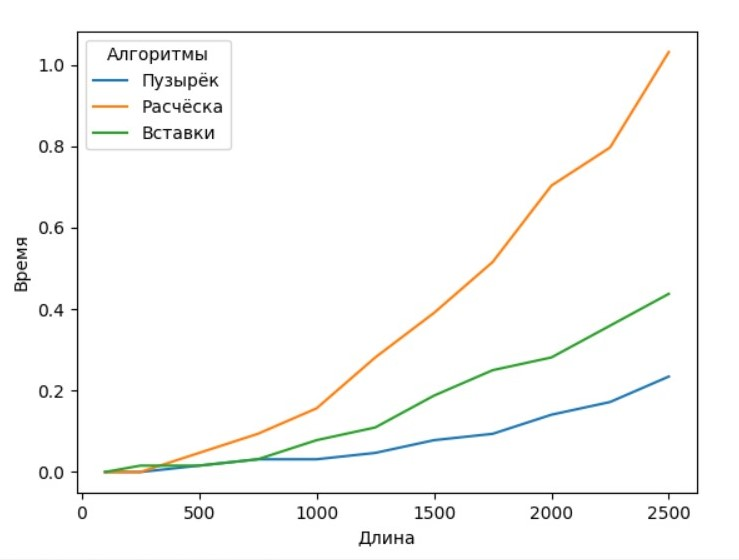
\includegraphics[scale=0.7]{res_graph}}
	\caption{График зависимости времени сортировки от размера массива}
\end{figure}

\section{Вывод}
В результате эксперимента было получено, что на массивах длинной 0 до 2500 элементов, алгоритм сортировки ''пузырьком'' работает быстрее алгоритмов ''пузырька'' и ''расчёски'' в 1.8 и 4.4 раза соответсвтенно. В результате можно сделать вывод, что для сортировки массивов предпочтительно использовать реализованный в данной лабораторной работе алгоритм ''пузырька''.